\documentclass[12pt]{article}
\usepackage{a4wide}
\usepackage{latexsym}
\usepackage{amssymb}
\usepackage{epic}
\usepackage{amsmath}
\usepackage{graphicx}
\usepackage{comment}
\usepackage{graphicx}
\usepackage{tikz}
%\pagestyle{empty}
\newcommand{\tr}{\mbox{\sf true}}
\newcommand{\fa}{\mbox{\sf false}}
\newcommand{\bimp}{\leftrightarrow}

\begin{document}
\section*{Automated Reasoning\\Assignment 1}

\begin{center}
Wouter Geraedts (s0814857) \\
Judith van Stegeren (s3014827)\\
\end{center}

\vspace{8mm}

\subsection*{Trucks and pallets}
The problem: find a way to load pallets of different objects onto 6 trucks, while adhering to various constraints. 
Investigate the maximum number of pallets of prittles that can be delivered, 
and show how for that number all pallets may be divided over the six trucks.

We have generalized the problem in the following way: given $t$ trucks with a capacity of $c$ that can carry at most $p$ pallets, an array \texttt{amount} of numbers of pallets of nuzzles, skipples, crottles and dupples and an array \texttt{weight} of the weight of a pallet of each of these items, maximize the number of pallets of prittles that can be delivered.
Note that throughout the text we use the number `$0$' (the index corresponding to nuzzles), the full object name `\texttt{nuzzles}' or the single letter `\texttt{n}' interchangably, to increase readability.

We start out by introducing our representation. We have a function 
\[\texttt{Pallets :: Int -> Int -> Int}\]
\texttt{Pallets t o} returns the number of pallets of object \texttt{o} that truck \texttt{t} is carrying.

Trucks cannot carry a negative amount of pallets:
\[ \bigwedge_{0 \le \texttt{i} < t} \bigwedge_{0 \le \texttt{j} < o} \texttt{Pallets i j} \ge 0 \]

Trucks cannot carry more than $p$ pallets:
\[ \bigwedge_{0 \le \texttt{i} < t} ~ ( \sum_{0 \le \texttt{j} < o} \texttt{Pallets i j} ) \le p \]

Each pallet of object \texttt{o} weighs \texttt{weight[o]} kg. Trucks cannot carry more than the maximum weight of $c$ kg:
\[ \bigwedge_{0 \le \texttt{i} < t} ~ (\sum_{0 \le \texttt{j} < o} \texttt{Pallets i j} \cdot \texttt{weight[j]}) \le c \]
Prittles and crottles are not allowed in the same truck. In other words, for every truck \texttt{t} it should not be possible that \texttt{(Pallets t prittles)} and \texttt{(Pallets t crottles)} are both greater than 0:
\[ \bigwedge_{0 \le \texttt{i} < t} \neg \left(( \texttt{Pallets i prittles} > 0) \wedge (\texttt{Pallets i crottles} > 0 )\right)\]

There can be at most 2 trucks carrying skipples. To be able to express this constraint, we first need to count the number of trucks carrying skipples. We introduce a variable \texttt{skt} to count the number of skipple-carrying trucks. We calculate the value of this integer by summing over all trucks \texttt{t} with a simple if-then-else-statement in yices: 
\[ \texttt{skt} = \sum_{0\le \texttt{i} < t} \texttt{(ite (> (Pallets i skipples) 0) 1 0)}\]

Now we can easily express the constraint by adding the following to our formula:
\[ \texttt{skt} \le 2 \]

We have to deliver \texttt{amount[o]} pallets of object \texttt{o}. Finally we assert that all pallets in the delivery should be loaded onto the trucks:

\[ \bigwedge_{0 \le \texttt{i} < o} \sum_{0 \le \texttt{j} < t} \texttt{Pallets j o} = \texttt{amount[o]}\]

We fill in a number for \texttt{amount[prittles]} and see if the formule is satisfiable. We use binary search to find the maximum number of pallets of prittles that we can deliver.
The formula was satisfiable when \texttt{amount[prittles]} was equal to 20.
We show the assignment found by the solver in figure \ref{fig:sub1table}.
Since this brings the total amount of delivered pallets to 47 and the maximum number of pallets we can carry with the six trucks is 48, this seems like a plausible solution.

\begin{figure}[h]
    \begin{center}
        \begin{tabular}{r|ccccc}
        truck & \texttt{n} & \texttt{p} & \texttt{s} & \texttt{c} & \texttt{d} \\\hline
        $t_0$ & 1 & 0 & 7 & 0 & 0 \\
        $t_1$ & 0 & 0 & 0 & 5 & 2 \\
        $t_2$ & 2 & 6 & 0 & 0 & 0 \\
        $t_3$ & 0 & 0 & 0 & 5 & 3 \\
        $t_4$ & 0 & 8 & 0 & 0 & 0 \\
        $t_5$ & 1 & 6 & 1 & 0 & 0 \\\hline
        total & 4 & 20 & 8 & 10 & 5 \\
        \end{tabular}
    \end{center}
    \caption{Assignment of pallets to trucks for an optimal solution.}
    \label{fig:sub1table}
\end{figure}

\subsection*{Rectangles and squares}
The problem: we have a list of $n$ shapes (rectangles and squares) 
$s_0\dots s_{n-1}$ of dimensions width$(s_i)$ and height$(s_i)$.
%of width \texttt{W(s_i)} and height \texttt{H(s_i)}.
We also have a large square of width $b$.% and height \texttt{bound_y}. 
We want to find a way to place all shapes within the bounding square 
without any shape overlapping the other.

We start out by defining 4 functions. 
We need these for our representation.

\begin{enumerate}
\item the function \texttt{W :: Int -> Int} that returns the width of a shape.
\item the function \texttt{H :: Int -> Int}  that returns the height of a shape.
\item the function \texttt{X :: Int -> Int} that returns the x-coordinate of the upper-left-point of a shape.
\item the function \texttt{Y :: Int -> Int} that returns the y-coordinate of the upper-left-point of a shape.
\end{enumerate}

We need \texttt{W} and \texttt{H} to define the actual size of all shapes,
and \texttt{X} and \texttt{Y} to represent where the shapes are placed in the big square.

In this particular example, $s_0$ and $s_1$ are the squares of sizes 4 and 6, and $s_2 \dots s_9$ are the rectangles with length $2 \dots 9$.

The first thing we have to put in the formula, is that all shapes can be placed either horizontally or vertically in the square.
In other words, for all shapes we have that either 
$(\texttt{W i}) = \text{width}(s_i) \text{~and~} (\texttt{H i}) = \text{height}(s_i)$ or 
$(\texttt{W i}) = \text{height}(s_i) \text{~and~} (\texttt{H i}) = \text{width}(s_i)$:

\[ \bigwedge_{0 \le i < n}
(\texttt{W i}) = \text{width}(s_i) \wedge (\texttt{H i}) = \text{height}(s_i) \oplus
(\texttt{W i}) = \text{height}(s_i) \wedge (\texttt{H i}) = \text{width}(s_i)
\]

Furthermore, all shapes must stay within the bounds of the big square, ie. their X and Y coordinates must be somewhere between 0 and $b$.

\[ \bigwedge_{0 \le i < n}
(\texttt{X i}) \ge 0 \wedge
(\texttt{Y i}) \ge 0 \wedge
(\texttt{X i})+(\texttt{W i}) \le b \wedge
(\texttt{Y i})+(\texttt{H i}) \le b
\]

We also don't want any of the shapes to overlap.
In order to check whether two shapes $s_i$ and $s_j$ overlap, we first define an inclusion-relation:
\[ s_i \in s_j \]
On the X-axis, $s_j$ is (partially) included in shape $s_i$, in other words $s_i \in_{\texttt{X}} s_j$, iff either:

% X_i <= X_j && X_j < X_i + W_i
\begin{center}
    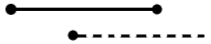
\includegraphics[width=5cm]{bounds1.png}
\end{center}
\[ (\texttt{X i}) \le (\texttt{X j}) ~\wedge~ (\texttt{X j}) < (\texttt{X i}) + (\texttt{W i}) \]
or
% X_i < X_j + W_j && X_j + W_j <= X_i + W_i
\begin{center}
    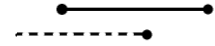
\includegraphics[width=5cm]{bounds2.png}
\end{center}
\[ (\texttt{X i}) < (\texttt{X j}) + (\texttt{W j}) ~\wedge~ (\texttt{X j}) + (\texttt{W j}) \le (\texttt{X i}) + (\texttt{W i}) \]

The same relation holds for the Y-axis, thus $s_i \in_{\texttt{Y}} s_j$, when all $\texttt{X}$ variables are replaced by $\texttt{Y}$ variables.
The inclusion relation for two dimensions holds iff both formulas for both axis hold at the same time.

\[ s_i \in_{\texttt{XY}} s_j \iff s_i \in_{\texttt{X}} s_j \wedge s_i \in_{\texttt{Y}} s_j \]

We then define overlap as the symmetric inclusion relation:

\[ s_i \bowtie s_j \iff s_i \in_{\texttt{XY}} s_j ~\vee~ s_j \in_{\texttt{XY}} s_i \]

However, this overlap relation does not work as we would like.
For example, if a big square is covered by a rectangle like this:
\begin{center}
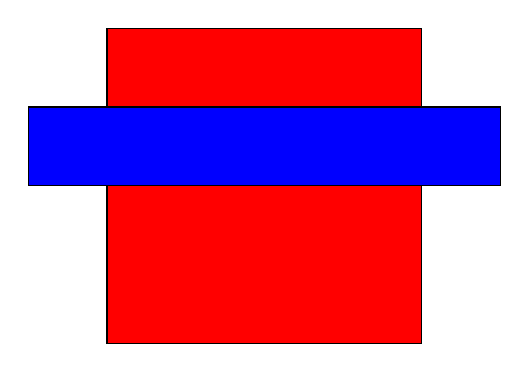
\begin{tikzpicture}[>=latex]
\draw[fill=red] (1,0) rectangle (5,4);
\draw[fill=blue] (0,2) rectangle (6,3);
\end{tikzpicture}
\end{center}

We clearly see that there is overlap, but the two objects do not include eachother as defined in our inclusion relation.
The overlap relation can be fixed by requiring a symmetric one-dimensional inclusion relation:
\[ s_i \bowtie s_j \iff (s_i \in_{\texttt{X}} s_j ~\vee~ s_j \in_{\texttt{X}} s_i) \wedge (s_i \in_{\texttt{Y}} s_j ~\vee~ s_j \in_{\texttt{Y}} s_i) \]
The `no overlap' constraint can then be formulated as:
\[ \neg \bigvee_{0 \le i < n} ~ \bigvee_{0 \le j < i} s_i \bowtie s_j \]
As the relation is symmetric, we only need to check half of the pairs of shapes.
Every shape also overlaps with itself, so we exclude the reflexive pairs of shapes as well.

We get the following pseudo-Yices after expanding these definitions:
\[
    \begin{array}{rlcl}
        \neg \bigvee_{0 \le i < n} ~ \bigvee_{0 \le j < i} & & & \\
            (~~~ & (~(\texttt{X i}) \le (\texttt{X j}) & \wedge & (\texttt{X j}) < (\texttt{X i}) + (\texttt{W i}) ) \\
            \vee & (~(\texttt{X i}) < (\texttt{X j}) + (\texttt{W j}) & \wedge & (\texttt{X j}) + (\texttt{W j}) \le (\texttt{X i}) + (\texttt{W i})~) \\
            \vee & (~(\texttt{X j}) \le (\texttt{X i}) & \wedge & (\texttt{X i}) < (\texttt{X j}) + (\texttt{W j}) ) \\
            \vee & (~(\texttt{X j}) < (\texttt{X i}) + (\texttt{W i}) & \wedge & (\texttt{X i}) + (\texttt{W i}) \le (\texttt{X j}) + (\texttt{W j})~) \\
            )~~~ & & & \\
     \wedge~(~~~ & (~(\texttt{Y i}) \le (\texttt{Y j}) & \wedge & (\texttt{Y j}) < (\texttt{Y i}) + (\texttt{H i}) ) \\
            \vee & (~(\texttt{Y i}) < (\texttt{Y j}) + (\texttt{H j}) & \wedge & (\texttt{Y j}) + (\texttt{H j}) \le (\texttt{Y i}) + (\texttt{H i})~) \\
            \vee & (~(\texttt{Y j}) \le (\texttt{Y i}) & \wedge & (\texttt{Y i}) < (\texttt{Y j}) + (\texttt{H j}) ) \\
            \vee & (~(\texttt{Y j}) < (\texttt{Y i}) + (\texttt{H i}) & \wedge & (\texttt{Y i}) + (\texttt{H i}) \le (\texttt{Y j}) + (\texttt{H j})~) \\
            )~~~ & & & \\
    \end{array}
\]

The SMT-solver found the following solution for the list of shapes given in the exercise and a large square of 10 by 10:\\
\begin{center}
    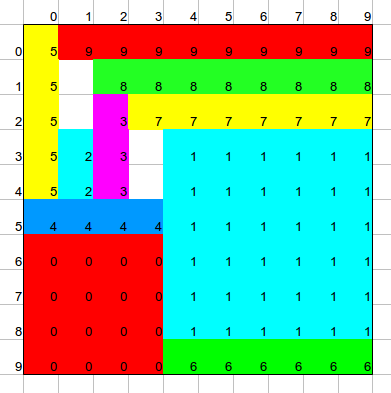
\includegraphics[width=12cm]{rectangles.png}
\end{center}

The second part of the exercise was proving that for every solution, 
the rectangles of length 8 and 9 are placed in parallel, 
but not all non-square rectangles. 

To prove this statement, we include rules in the formula 
that state the negation of the statement we have to prove.
If the SMT-solver then tells us that the formula is unsatisfiable, we know that the statement must be true for every solution. 
%Note that the negation of the statement is equivalent to "8 and 9 are not placed or all non-square rectangles are placed in parallel".

%To prove:
%8 and 9 placed in parallel AND not all rectangles in parallel
%NOT ( 8 and 9 placed in parallel AND not all rectangles in parallel )
%(NOT 8 and 9 placed in parallel OR NOT NOT all rectangled in parallel )

The rectangles with length 8 and 9 are placed in parallel, ie. they are either both placed horizontally or vertically:
(\texttt{(W 8)} = width($s_8) \wedge$ \texttt{(H 8)} = height($s_8) \wedge$
\texttt{(W 9)} = width($s_9) \wedge$ \texttt{(H 9)} = height($s_9))
\vee$\\
(\texttt{(W 8)} = height($s_8) \wedge$ \texttt{(H 8)} = width($s_8) \wedge$
\texttt{(W 9)} = height($s_9) \wedge$ \texttt{(H 9)} = width($s_9$))\\

Not all non-square rectangles are placed in parallel, ie. it is not the case that they are either all placed horizontally or all placed vertically:
\[
\neg
\left(
\bigvee_{2 \le i \le 9}
\left( 
\texttt{(W i)} = \text{width}(s_i) \wedge \texttt{(H i)} = \texttt{height}(s_i)
\right)
\oplus
\bigvee_{2 \le i \le 9}
\left(
\texttt{(W i)} = \text{height}(s_i) \wedge \texttt{(H i)} = \text{width}(s_i)
\right)
\right)
\]

\subsection*{Scheduling of jobs}
The problem: schedule twelve jobs with different running times, while adhering to a list of constraints.
Investigate the minimal running time needed to complete all jobs.
Our solution works for a arbitrary number of jobs.
We want to schedule $j$ jobs numbered from 1 to $j$.
The running time for job $i$ is $rt_i = i+5$.

Our representation is as follows.
We have a timeline of length $T$.
For every moment in time, we have a status code for every job: it is either ready (0), running (1) or finished (2). 
For this we have the function 
\[\texttt{Status :: Int -> Int -> Int}\]
\texttt{Status 1 10 2} means that job 1 at timeframe 10 is finished. 

The job status must be either 0, 1 or 2, for all jobs and moments in time:
\[ \bigwedge_{0 \le \texttt{t} < T} ~ \bigwedge_{0 \le \texttt{i} < j} \texttt{Status i t} \ge 0\wedge \texttt{Status i t} \le 2\]

We now want to specify the correct behaviour for each job. 
Since the running time for each job $i$ is $rt_i$ and we want it to be finished before or on timeframe $T-1$ (the end of the timeline), we have to start job $i$ at timeframe $T - rt_i$ at the latest.
We take $st_i$ as the starting time of job $i$, with $0 \le st_i < lt_i$ and $lt_i = T-rt_i$.

Before a job starts (1), it must be ready (0):
\[ \bigwedge_{0 \le \texttt{tt} < st_i} \texttt{Status i tt} = 0 \]

We want the jobs to run without interrupt.
In other words, if a job has started, it will not stop until it is finished. 
If job $i$ starts at timeframe $st_i$, it keeps running in timeframes $st_i \dots (st_i + rt_i)$.
\[ \bigwedge_{0 \le \texttt{rt} < rt_i} \texttt{Status i (st+rt)} = 1 \]

If the job is done running, it is finished and it will stay finished for the remainder of the timeframes, starting at timeframe $st_i + rt_i$.
\[ \bigwedge_{0 \le \texttt{tt} < T-st-rt_i} \texttt{Status i tt} = 2 \]

If we put these three conditions together, we get:
\[ \begin{array}{rll}
    \bigwedge_{0 \le \texttt{i} < j} \bigvee_{0 \le \texttt{st} < lt_i} \left( \right.&& \\
    & \bigwedge_{0 \le \texttt{tt} < st} & \texttt{Status i tt} = 0 ~ \wedge \\
    & \bigwedge_{0 \le \texttt{tt} < rt_i} & \texttt{Status i st+tt} = 1 ~ \wedge \\
    & \bigwedge_{0 \le \texttt{tt} < T-st-rt_i} & \texttt{Status i tt} = 2 \\
\left. \right)
\end{array} \]

Now we have a number of job specific constraints. 
If we want to express that job a is only allowed to start if job b and c have finished, we write: 
\[ \bigwedge_{0 \le \texttt{tt} < T} (\texttt{Status a tt} = 1) \rightarrow (\texttt{Status b tt} = 2 \wedge \texttt{Status c tt} = 2) \]

Job 3 may only start if job 1 and 2 have finished.
\[ \bigwedge_{0 \le \texttt{tt} < T} (\texttt{Status 3 tt} = 1) \rightarrow (\texttt{Status 1 tt} = 2 \wedge \texttt{Status 2 tt} = 2) \]
Job 5 may only start if job 3 and 4 have finished.
\[ \bigwedge_{0 \le \texttt{tt} < T} (\texttt{Status 5 tt} = 1) \rightarrow (\texttt{Status 3 tt} = 2 \wedge \texttt{Status 4 tt} = 2) \]
Job 7 may only start if job 3, 4 and 6 have finished.
\[ \bigwedge_{0 \le \texttt{tt} < T} (\texttt{Status 7 tt} = 1) \rightarrow (\texttt{Status 3 tt} = 2 \wedge \texttt{Status 4 tt} = 2 \wedge \texttt{Status 6 tt} = 2) \]
Job 9 may only start if job 5 and 8 have finished.
\[ \bigwedge_{0 \le \texttt{tt} < T} (\texttt{Status 9 tt} = 1) \rightarrow (\texttt{Status 5 tt} = 2 \wedge \texttt{Status 8 tt} = 2) \]
Job 11 may only start if job 10 has finished.
\[ \bigwedge_{0 \le \texttt{tt} < T} (\texttt{Status 11 tt} = 1) \rightarrow (\texttt{Status 10 tt} = 2\]
Job 12 may only start if job 9 and 11 have finished.
\[ \bigwedge_{0 \le \texttt{tt} < T} (\texttt{Status 12 tt} = 1) \rightarrow (\texttt{Status 9 tt} = 2 \wedge \texttt{Status 11 tt} = 2) \]

Another constraint is that job 8 may not start earlier than job 5, in other words, we want that if job 5 starts running, job 8 is either running as well or already finished:
\[ \bigwedge_{0 \le \texttt{tt} < T} (\texttt{Status 5 tt} = 1) \rightarrow (\texttt{Status 8 tt} > 0) \]

For job 5, 7 and 10 we have that no two of these job may be running at the same time. 
We introduce a variable $nr_t$ to count the number of running jobs 5, 7 and 10 in timeframe $t$.
We calculate the value of this integer by summing over jobs 5, 7 and 10 with a simple if-then-else-statement in yices: 
\[ nr_t = \sum_{i \in \{5,7,10\}} \texttt{ite (= 1 (Status i t)) 1 0} \]
Now we can enforce the constraint by counting the number of running jobs 5, 7 and 10 in each timeframe, 
and stating that this number is not allowed to be greater than 1. 
\[ \bigwedge_{0 \le t < T} nr_t \le 1\]

We filled in a value for the variable time (the length of the timeline) 
and asked the SMT-solver whether the formule was satisfiable. 
We used binary search to find the minimal number of time frames needed to schedule all jobs. 
We found the value 59. 
Below is a Gant chart that shows us how the jobs were scheduled within 59 time frames:
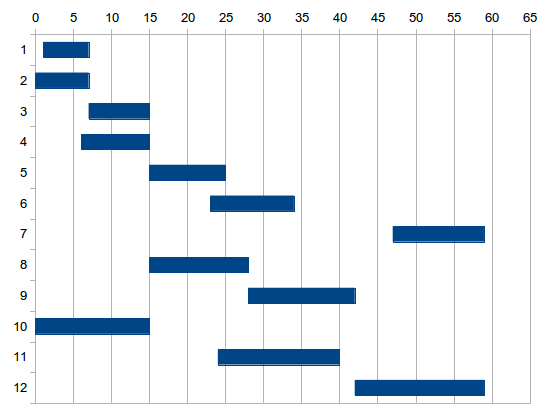
\includegraphics[width=15cm]{gantchart.png}

\subsection*{Computation steps}
We start with a set of $N$ variables $a_1, \dots, a_N$ with initial values $1 \dots N$.
%For all variables except $a_1$ and $a_N$, it is possible to either do nothing, or assign a new value to the variable:
We want to obtain a variable with the value 157 in a number of steps. 
In such a step, we choose a variable $a_v$ with $1 < v < N$ and assign it a new value:
\[ a_v = a_{v-1} + a_{v+1} \]
We want to find the minimum number of these steps required to get a variable with the value 157.
We compute this by fixing the number of steps $T$, and then defining a function
\[\texttt{A :: Int -> Int -> Int}\]
such that \texttt{A v t} is the value of variable $a_v$ after $t$ steps.

First we define the initial value for all variables:
\[ \bigwedge_{1 \le \texttt{v} \le N} \texttt{A v 0} = \texttt{v} \]
Then we define the steps allowed for each variable.
The $t^\mathtt{th}$ step can be done by precisely one variable $a_v$ in $\{ a_2, \cdots, a_{N-1} \}$.
This step is done by updating this variable:
\[\texttt{A v (t+1)} = \texttt{A (v-1) t} + \texttt{A (v+1) t}\]
And all other variables must remain unchanged:
\[\bigwedge_{ \texttt{u} \in \{1, \cdots, N\} \setminus \{ \texttt{v} \} } \texttt{A u (t+1)} = \texttt{A u t}\]

This can be done for any step $t$, thus this entire section can be written down with:
\[
    \bigwedge_{0 \le \texttt{t} < T}
    \bigvee_{1 < \texttt{v} < N}
        \left (\texttt{A v (t+1)} = \texttt{A (v-1) t} + \texttt{A (v+1) t} \right)
        ~\wedge~
        \left( \bigwedge_{ \texttt{u} \in \{1, \cdots, N\} \setminus \{ \texttt{v} \} } \texttt{A u (t+1)} = \texttt{A u t} \right)
\]

Finally we define the end-goal:
\[ \bigvee_{1 \le \texttt{v} \le N} \texttt{A v T} = 157 \]

%To find the minimum number of steps required, we use binary search on the number of steps $T$.
To minimize the number of steps, we use binary search on $T$.
Binary search is applicable because of the following:
if a variable $a_v$ has the value 157 after $t$ steps, the SMT-solver can pick a variable $a_w$ with $v \ne w$ for all subsequent steps.
In other words, 
if the SMT-solver finds that the formula is satisfiable for t steps, 
the formula is also satisfiable for a larger number of steps.

%Because when a variable $v$ has reachbed the value 157 after $T$ steps, in subsequent steps, the SMT-solver can always pick a variable that does not have the value 157.
%Since the value of variable $v$ then remains unchanged, the formula is also satisfiable for more than $T$ steps.
%Thus binary search is applicable in this case.

Our algorithm for binary search concludes that the problem can be solved in at least 10 steps.

\end{document}
